\documentclass[10pt, a4paper]{article}
\usepackage[toc,page]{appendix}
\usepackage{indentfirst}
\usepackage{arydshln} % for dashed line in tabular configuration
\usepackage{afterpage}
\usepackage{pdflscape}

\usepackage{hyperref}
\usepackage[style=authoryear-comp, sorting=nyt, maxcitenames=2, maxbibnames=99, firstinits=true, hyperref=true, dashed=false, uniquename=false, uniquelist=false, backend=biber]{biblatex}
% maxcitenames working for inside article
% maxbibnames working for the printbibliography
% firstinits=true making the last name to the .

%% \usepackage[style=authoryear-comp, sorting=nyt, maxcitenames=2, backend=biber]{biblatex}

\renewbibmacro{in:}{}
\renewcommand\bibfont{\small}
\addbibresource{Brownian_dynamics.bib}
% \addbibresource{reference.bib}
% \addbibresource{trappe.bib}

\usepackage{amsmath,amssymb, mathrsfs}
\usepackage{xcolor, graphicx, epstopdf}
\usepackage{amsthm}
\newtheorem{thm}{Theorem}
\newtheorem{lemma}{Lemma}
\newtheorem{mydef}{Definition}
\title{Short Notes for Brownian Dynamics with Elastic Dumbbells}
\author{Gun Woo Park}
\linespread{1.3}
\addtolength{\hoffset}{-1.5cm}
\addtolength{\textwidth}{3cm}
\addtolength{\voffset}{-1.5cm}
\addtolength{\textheight}{3cm}

% From here, listing for source code

\usepackage{listings}
\usepackage{courier}
\lstset{language=C++,
  basicstyle=\ttfamily,
  keywordstyle=\color{blue}\ttfamily,
  stringstyle=\color{red}\\ttfamily,
  commentstyle=\color{green}\ttfamily
  % breakline=true
  % morecomment=[1][\color{magenta}]{\#}
}
\lstset{language=Python,
  basicstyle=\ttm,
  otherkeywords={self},
  keywordstyle=\ttb\color{deepblue},
  emph={MyClass,__init__},
  emphstyle=\ttb\color{depred},
  stringstyle=\color{deepgreen},
  frame=tb
  % showstringspace=false
}
\lstset{
         basicstyle=\footnotesize\ttfamily, % Standardschrift
         numbers=left,               % Ort der Zeilennummern
         numberstyle=\color{brown}\tiny,          % Stil der Zeilennummern
         %stepnumber=2,               % Abstand zwischen den Zeilennummern
         numbersep=5pt,              % Abstand der Nummern zum Text
         tabsize=2,                  % Groesse von Tabs
         extendedchars=true,         %
         breaklines=true,            % Zeilen werden Umgebrochen
         keywordstyle=\color{blue},
    		frame=b,         
%        keywordstyle=[1]\textbf,    % Stil der Keywords
%        keywordstyle=[2]\textbf,    %
%        keywordstyle=[3]\textbf,    %
%        keywordstyle=[4]\textbf,   \sqrt{\sqrt{}} %
         stringstyle=\color{black}\ttfamily, % Farbe der String
         showspaces=false,           % Leerzeichen anzeigen ?
         showtabs=false,             % Tabs anzeigen ?
         xleftmargin=17pt,
         framexleftmargin=17pt,
         framexrightmargin=5pt,
         framexbottommargin=4pt,
         %backgroundcolor=\color{lightgray},
         showstringspaces=false      % Leerzeichen in Strings anzeigen ?        
 }
%  \lstloadlanguages{% Check Dokumentation for further languages ...
%          %[Visual]Basic
%          %Pascal
%          %C
%          C++,
%          Python
%          %XML
%          %HTML
%    %Java
%  }
  %\DeclareCaptionFont{blue}{\color{blue}} 

  %\captionsetup[lstlisting]{singlelinecheck=false, labelfont={blue}, textfont={blue}}
  \usepackage{caption}
\DeclareCaptionFont{white}{\color{white}}
\DeclareCaptionFormat{listing}{\colorbox[cmyk]{0.43, 0.35, 0.35,0.01}{\parbox{\textwidth}{\hspace{15pt}#1#2#3}}}
\captionsetup[lstlisting]{format=listing,labelfont=white,textfont=white, singlelinecheck=false, margin=0pt, font={bf,footnotesize}}

\begin{document}
\maketitle 
%% \section{Coupled Oscillator}
%% \section{Langevin Equation for Rigid Body}

% \section{Preface}
% The aim of this study is for interpretation of supramolecular solution that provide unusual properties such as report of \textcite{Suzuki:2012gf} that related with Hydrophobically modified Ethoxylated uRethane (HEUR) solution. The detail explanation for HEUR solution should be refer following references: \textcite{Suzuki:2013kk, Uneyama:2012ge, Suzuki:2012gf}. This document is for methodological development in order to interpretate complicated system based on Brownian dynamics. 

% For shortly, following is directions for evolution equation in dimensionless form:
% \begin{enumerate}
% \item Linear dumbbell model with simple Euler integrator and simple Wiener process: equation \eqref{eq:dimensionless_update_position}.
% \item Non-linear dumbbell model: TBD
% \item Rouse segments: TBD
% \end{enumerate}

\part{Simple Brownian Motion for Beads with Repulsion}
\section{Basic Fomular}
The evolution equation is given by
\begin{equation}
\frac{\partial \mathbf{r}}{\partial t} = \frac{1}{\zeta}\left(\sum \mathbf{F}^{(r)} + \mathbf{F}^{(s)}\right),
\end{equation}
where $\mathbf{F}^{(r)}$ is repulsive force and $\mathbf{F}^{(s)}$ is random force contribution. With simple Euler approach, we can represent the given evolution equation as
\begin{equation}
\mathbf{r}(t + \delta t) = \mathbf{r}(t) + \frac{1}{\zeta}\sum\mathbf{F}^{(r)}(t)\delta t + \delta \mathbf{r},\label{eq:update_position}
\end{equation}
where stochastic step, $\delta \mathbf{R}$ is defined by
\begin{equation}
\delta \mathbf{r} = \frac{1}{\zeta}\int_t^{t+\delta t}\mathbf{F}^{(s)}(t')dt'.\label{eq:stochastic_step}
\end{equation}

For convenience, let $\mathbf{r}_{ij} = \mathbf{r}_j - \mathbf{r}_i$. When distance between two micelles, $\lvert\mathbf{r}_{ij}\rvert$ are lesser than the diameter of single micelle, $R_0$, the repulsive force is defined by
\begin{equation}
\mathbf{F}^{(r)}(\mathbf{r}_i, \mathbf{r}_j) = \mathbf{F}^{(r)}(\mathbf{r}_{ij}) = -C\frac{k_BT}{R_0}\left(1 - \frac{\mathbf{r}_{ij}^2}{R_0^2}\right)\hat{\mathbf{r}}_{ij} \label{eq:force_repulsion}
\end{equation}
where hat denote directional vector, $R_0$ denote expected size for micelle, and non-dimensional parameter $C$ is given by
\begin{equation}
C = \frac{9}{\pi}n_p^2N^{0.2}
\end{equation}
with number of polymer in micelle, $n_p$, and Kuhn number for each polymer, $N$.


\section{Wiener Process for Random Force Contribution}

Define Wiener process as
\begin{equation}
\mathbf{W}(t) = \mathscr{W}\left[\mathbf{F}^{(s)}(t')\right] \equiv \int_0^{t} \mathbf{F}^{(s)}(t')dt',
\end{equation}
the stochastic step, $\delta \mathbf{r}$, is represented by the increment for Wiener process:
\begin{equation}
\zeta \delta \mathbf{r} = \mathbf{W}(t+\delta t) - \mathbf{W}(t) \equiv \Delta \mathbf{W}(\delta t).
\end{equation}
Using simple Euler integrator, the increment for Wiener process has property \parencite{GREINER:1988cq}:
\begin{equation}
\langle (\Delta\mathbf{W}(\delta t))^2 \rangle = 2\zeta k_BT \delta t\quad\textrm{with }\Delta \mathbf{W}(\delta t) \sim \mathscr{N}(0, 2\zeta k_BT\delta t),\label{eq:increment_Wiener_process}
\end{equation}
where $\mathscr{N}(\mu, \sigma^2)$ denote normal distribution with mean $\mu$ and variance $\sigma^2$.


\section{Non-dimensionalization (basic)}
Since the given micelle size is fixed as $R_0$, it is appropriate to set characteristic length, $l_c$, as $R_0$. Then, we can define characteristic time as
\begin{equation}
t_c = \frac{\zeta R_0^2}{k_BT}.\label{eq:characteristic_time}
\end{equation}
Note that
\begin{equation}
[t_c] = \frac{[\zeta][R_0^2]}{[k_BT]} = \frac{M\cdot T^{-1} L^2}{M\cdot L^2\cdot T^{-2}} = T.
\end{equation}

From dimensionality for increment of Wiener process, we can define dimensionless Gaussian noise $\tilde{\mathbf{R}}\sim\mathscr{N}(0,1)$  as
\begin{equation}
\Delta \mathbf{W} = \sqrt{2\zeta k_BT\delta t}\tilde{\mathbf{R}}.
\end{equation}
Note that the previous condition is equivalent to the $\tilde{\mathbf{R}}$ is following uniform distribution with the interval $[-\sqrt{3}, \sqrt{3}]$ because the variance of it becomes $(\sqrt{3}+\sqrt{3})^2/12 = 1$. 

Finally, we have non-dimensional Euler integrator from Eq. \label{eq:update_position}:
\begin{equation}
\tilde{\mathbf{r}}(\tilde{t} + \delta \tilde{t}) = \tilde{\mathbf{r}}(\tilde{t}) + \sum_{i,j}\tilde{\mathbf{F}}^{(r)}(\tilde{\mathbf{r}}_i, \tilde{\mathbf{r}}_j)\delta \tilde{t} + \tilde{\mathbf{F}}^{(s)}\sqrt{\delta\tilde{t}},
\end{equation}
with
\begin{align}
\tilde{\mathbf{F}}^{(r)}(\tilde{\mathbf{r}}_i, \tilde{\mathbf{r}}_j) &= -C\left(1-\tilde{\mathbf{r}}_{ij}^2\right)\frac{\tilde{\mathbf{r}}_{ij}}{\tilde{r}_{ij}}\\
\tilde{\mathbf{F}}^{(s)} &= \sqrt{2}\tilde{\mathbf{R}}
\end{align}

Note that if we want the uniform distribution from -1 to 1 for random noise, we can replace the random potential as
\begin{equation}
\tilde{\mathbf{F}}^{(s)} = \sqrt{2\times 12}\tilde{\mathbf{R}}'.
\end{equation}

\section{Non-dimensionalization with prefactor C}
Appropriate non-dimensionalization should made order of unity for the reduced (basic) variables. That means, the time scale should be involved the stifness for each potential, i.e., repulsive potential on this article. So, re-defined characteristic time becomes
\begin{equation}
t_c = \frac{\zeta R_0^2}{k_BT}\frac{1}{C},\label{eq:characteristic_time_C}
\end{equation}
while characteristic length is given constant, $R_0$.
Then, we have
\begin{equation}
\tilde{\mathbf{r}}(\tilde{t} + \delta \tilde{t}) = \tilde{\mathbf{r}}(\tilde{t}) + \sum_{i,j}\tilde{\mathbf{F}}^{(r)}(\tilde{\mathbf{r}}_i, \tilde{\mathbf{r}}_j)\delta \tilde{t} + \tilde{\mathbf{F}}^{(s)}\sqrt{\delta\tilde{t}},
\end{equation}
with
\begin{align}
\tilde{\mathbf{F}}^{(r)}(\tilde{\mathbf{r}}_i, \tilde{\mathbf{r}}_j) &= -\left(1-\tilde{\mathbf{r}}_{ij}^2\right)\frac{\tilde{\mathbf{r}}_{ij}}{\tilde{r}_{ij}}\\
\tilde{\mathbf{F}}^{(s)} &= \sqrt{\frac{2}{3}}\tilde{\mathbf{R}}
\end{align}
On this regards, the repulsive potential contribution is following
\begin{equation}
U(\mathbf{r}_i, \mathbf{r}_j) = U(\mathbf{r}_{ij}) = \frac{1}{3}\left(1 + \tilde{\mathbf{r}}_{ij}\right)^2(2 + \tilde{\mathbf{r}}_{ij}).
\end{equation}

It is noteworthy that the repulsive coeffficient, $C$, effect to the system. If it is order of unity, both of repulsive and random forces are comparable. If $C\sim 5900$, the contribution for random force is $\sim 1/77$.

From now on, the dimensionless scheme is following the prefactor one.

\section{Numerical Computing}
\subsection{Development Environment}
The developed package is written by C++ integrated with Intel Compiler 


\section{Post-Processing}
\subsection{Identification of Equilibrium, Pure Brownian Simulation}

\subsection{Identification of Equilibrium, Repulsive Potential}




\part{van den Brule's Approach for Transient Networks System}
\subsection{Introduction}
This approach is based on the paper \textcite{VandenBrule:1995fq} that provide interpretation for the flow effect to the transient network system based on Brownian dynamics simulation with dumbbell model.

The basic evolution equation has the form of
\begin{equation}
\frac{\partial \mathbf{r}(t)}{\partial t} = \left.\frac{\partial \mathbf{r}}{\partial t}\right\rvert_{t=0} + \mathbf{k}\cdot\mathbf{r} + \frac{1}{\zeta} \left(\mathbf{F}^{(c)} + \sum\mathbf{F}^{(r)} + \mathbf{F}^{(r)}\right),
\end{equation}
where super scripts for forces (c), (r), and (s) refer connector, repulsion, and solution contribution, respectively.  Then, simple Euler integrator \textcite{GREINER:1988cq} gave us the evolution equation for position as follow:
\begin{equation}
\mathbf{r}(t + \delta t) = \mathbf{r} + \mathbf{v}_0 \delta t + \mathbf{k}\cdot\mathbf{r} \delta t + \frac{1}{\zeta}\left(\mathbf{F}^{(c)} + \sum \mathbf{F}^{(r)}\right)\delta t + \delta \mathbf{r},\label{eq:update_position_Brule}
\end{equation}
where the stochastic step, $\delta \mathbf{r}$, is the same with Eq. \eqref{eq:stochastic_step}.
Note that the methodology for the previous section is based on the approaches on \textcite{VandenBrule:1995fq}, that is almost all of the methdology is same including Wiener process. So, the exact expression for the stochastic step and Wiener process refer the previous section or \textcite{VandenBrule:1995fq, GREINER:1988cq}.

The simple harmonic potential is used for spring between beads, that is Gaussian spring:
\begin{equation}
\mathbf{F}^{(c)}(\mathbf{r}_i, \mathbf{r}_j) = \mathbf{F}^{(c)}(\mathbf{r}_{ij}) = H\mathbf{r}_{ij},
\end{equation}
where $H$ is given spring constants. 

In the case for repulsive potential, simple linear repulsion is used:
\begin{equation}
\mathbf{F}^{(r)}(\mathbf{r}_i, \mathbf{r}_j) = \mathbf{F}^{(r)}(\mathbf{r}_{ij})=-F_0 \left(1 - \frac{2}{l_c}r_{ij}\right)\hat{\mathbf{r}}_{ij} \quad\textrm{for }r_{ij} < \frac{1}{2}l_c,
\end{equation}
where the $1/2l_c$ is choosen for effective length for repulsion.

\subsection{Non-dimensionalization}
Based on the elastic dumbbell model, the characteristic length is typically defined as
\begin{equation}
l_c^2 = \langle \mathbf{r}_{ij}^2 \rangle = \int \mathbf{r} P(\mathbf{r}) d\mathbf{r} = \frac{3k_BT}{H}.
\end{equation} 
For the time scale, typical relaxation time for Hookean elastic dumbbell is used \textbf{(need calculation)}:
\begin{equation}
t_c = \frac{\zeta}{4H}.
\end{equation}
Then, equation \eqref{eq:update_position_Brule} becomes
\begin{equation}
\tilde{\mathbf{r}}(\tilde{t} + \delta \tilde{t}) = \tilde{\mathbf{r}}(\tilde{t}) + \tilde{\mathbf{v}}_0\delta t + \tilde{\mathbf{k}}\cdot\tilde{\mathbf{r}}\delta\tilde{t} + \tilde{\mathbf{F}}^{(c)}(\tilde{\mathbf{r}}, \mathscr{C}(\tilde{\mathbf{r}})\delta\tilde{t} + \sum_{i,j}\tilde{\mathbf{F}}^{(r)}(\tilde{\mathbf{r}}_{i}, \tilde{\mathbf{r}}_{j})\delta \tilde{t} + \tilde{\mathbf{F}}^{(s)}\sqrt{\delta \tilde{t}},
\end{equation}
where $\mathscr{C}(\mathbf{r})$ denote set of index that connected with $\mathbf{r}$, and the forces are represented as following:
\begin{align}
\tilde{\mathbf{F}}^{(c)}(\tilde{\mathbf{r}}_{ij}) &= \frac{1}{4}\tilde{\mathbf{r}}_{ij} \\
\tilde{\mathbf{F}}^{(r)}(\tilde{\mathbf{r}}_{ij}) &= -C\left(1 - 2\tilde{r}_{ij}\right)\frac{\tilde{\mathbf{r}}_{ij}}{\tilde{r}_{ij}}\\
\tilde{\mathbf{F}}^{(s)}(t) &= \frac{1}{\sqrt{6}}\tilde{\mathbf{R}} = \sqrt{2}\tilde{\mathbf{R}}',
\end{align}
where the random vector $\tilde{\mathbf{R}}\sim\mathscr{N}(0, 1)$, i.e., uniform distribution on the interval $\left[-\sqrt{3}, \sqrt{3}\right]$, and $\tilde{\mathbf{R}}'$ is uniform distribution on the interval $[-1, 1]$.

\part{Some Notes for Langevin Dynamics and Rouse Models}
\section{Continuous Langevin Equation for Rouse Model}
Rouse model is simplified version to describe bead-spring model in effective medium, polymer melt in this case, that successfully describe the unentangled polymer dynamics in melt (or solution) state. Let assumed that the number of beads is sufficiently large that produce continuity.  From this perspective, the dynamics of such system can be represented by Langevin equation:
\begin{equation}
\frac{\partial}{\partial t}\mathbf{R}(n, t) = \int_{0}^{N}dm\, \mathbf{H}(n, m)\cdot\left(-\frac{\partial U}{\partial \mathbf{R}(m, t)} + \mathbf{f}(m, t)\right) + \frac{1}{2}k_BT\int_{0}^{N}dm\,\frac{\partial}{\partial \mathbf{R}(m, t)}\cdot\mathbf{H}(n, m),
\label{eq:Langevin_basic_continuous}
\end{equation}
with mobility tensor, $\mathbf{H}$ given by
\begin{equation}
\mathbf{V}(n,t) = \int_0^N dm\,\mathbf{H}(n,m)\cdot\mathbf{F}(m,t).
\end{equation}
and with spring potential for U. 
Since we already assumed that the beads and springs are dipped into the isotropic effective medium, without p
\begin{equation}
\mathbf{H}(n,m) = \frac{\delta(n,m)}{\zeta}\mathbf{I},
\end{equation}
that $\zeta$ is comes from the 
\begin{align}
\mathbf{H}(n,m) &= \frac{1}{\zeta}\delta(n,m)\mathbf{I}, \\
U &= \frac{3k_BT}{2b^2}\int_{0}^{N}dk\,\left(\frac{\partial \mathbf{R}(k, t)}{\partial k}\cdot\frac{\partial \mathbf{R}(k, t)}{\partial k}\right)
\end{align}
where Kronecker-delta function, $\delta_{i,j}$, on discrete version is replaced by Dirac-delta function, $\delta(x, y)$, with continuous variables.
Here $\mathbf{H}$ is refer for mobility tensor, and given by
On this regards, we have
% \begin{align}
% &\int_0^{N}dm\,\delta(n,m)\mathbf{I}\cdot\left[\frac{\partial}{\partial \mathbf{R}(m,t)}\int_0^{N}dn\,\left(\frac{\partial \mathbf{R}(n, t)}{\partial n}\cdot\frac{\partial \mathbf{R}(n, t)}{\partial n}\right)\right]\\
% =& \int_0^{N}dm\,\mathbf{I}\cdot\left[\frac{\partial}{\partial \mathbf{R}(m,t)}\left(\frac{\partial \mathbf{R}(m, t)}{\partial m}\cdot\frac{\partial \mathbf{R}(m, t)}{\partial m}\right)\right]
% \end{align}
Therefore, the detail version of equation \eqref{eq:Langevin_basic_continuous} is derived by
\begin{equation}
\frac{\partial}{\partial t}\mathbf{R}(n, t) = \frac{1}{\zeta}\left(-\frac{\partial U}{\partial \mathbf{R}(n, t)} + \mathbf{f}(n, t)\right)
\end{equation}
Note that
\begin{align}
\frac{\partial U}{\partial \mathbf{R}(n, t)} &= \frac{3k_BT}{2b^2}\frac{\partial}{\partial \mathbf{R}(n,t)}\int_0^N dk\,\left(\frac{\partial \mathbf{R}(k, t)}{\partial k}\cdot\frac{\partial \mathbf{R}(k, t)}{\partial k}\right)\\
% &= \frac{3k_BT}{2b^2}\int_0^N dk\,\frac{\partial n}{\partial \mathbf{R}(n,t)}\frac{\partial}{\partial n}\left(\frac{\partial \mathbf{R}(k, t)}{\partial k}\cdot\frac{\partial \mathbf{R}(k, t)}{\partial k}\right)\\
&= \frac{3k_BT}{2b^2}\int_0^N dk\,\frac{\partial n}{\partial \mathbf{R}(n,t)}\frac{\partial k}{\partial n}\frac{\partial}{\partial k}\left(\frac{\partial \mathbf{R}(k, t)}{\partial k}\cdot\frac{\partial \mathbf{R}(k, t)}{\partial k}\right)\\
&= \frac{3k_BT}{b^2}\int_0^N dk\,\frac{\partial n}{\partial \mathbf{R}(n,t)}\delta(k,n)\frac{\partial^2 \mathbf{R}(k, t)}{\partial k^2}\cdot\frac{\partial \mathbf{R}(k, t)}{\partial k}\\
% &= \frac{3k_BT}{b^2}\frac{\partial n}{\partial \mathbf{R}(n,t)}\frac{\partial \mathbf{R}(n, t)}{\partial n}\cdot\frac{\partial^2 \mathbf{R}(n, t)}{\partial n^2}\\
&= \frac{3k_BT}{b^2}\frac{\partial^2 \mathbf{R}(n, t)}{\partial n^2}
\end{align}
The continuous Langevin equation for Rouse model becomes
\begin{equation}
\frac{\partial}{\partial t}\mathbf{R}(n, t) = -\frac{3k_BT}{\zeta b^2}\frac{\partial^2 \mathbf{R}(n,t)}{\partial n^2} + \frac{1}{\zeta}\mathbf{f}(n,t)
\label{eq:Langevin_continuous_Rouse}
\end{equation}

\subsection{Eigenfunction Decomposition}
The idea of normal coordinate is simple: finding coordinate system based on eigenfunction that produce the differential equation to the linear equation. 
On this regards, we can consider linear integral transform, $\mathscr{L}$, that provide p- from n-coordinate system.
In this case, we can easily prove that the proposed transform is linear since the integration is linear. Note that since $\mathscr{L}$ is coordinate transform, there exist inverse transform $\mathscr{L}^{-1}$ that convert from p- to n-coordinate system as following manner:
\begin{equation}
\mathbf{X}(p, t) = \mathscr{L}\left[\mathbf{R}(n, t)\right]\quad\Leftrightarrow\quad\mathbf{R}(n, t) = \mathscr{L}^{-1}\left[\mathbf{X}(p, t)\right].
\label{eq:coordinate_transform}
\end{equation}
Let $\mathbf{X}(p,t)$ be transformed position vector for bead,
\begin{equation}
\mathbf{X}(p, t) \equiv \mathscr{L}\left[\mathbf{R}(n,t)\right] = \frac{1}{N} \int_0^N dn \,\phi(p, n)\mathbf{R}(n, t),
\end{equation}
where $\phi(p, n)$ is kernel function. 
Taking partial integration for the RHS of equation \eqref{eq:Langevin_continuous_Rouse}, we have
\begin{align}
  \mathscr{L}\left[\frac{\partial^2\mathbf{R}(n,t)}{\partial n^2}\right] &= \frac{1}{N}\left[ \left.\phi(p,n)\frac{\partial \mathbf{R}(n,t)}{\partial n}\right\rvert_{n=0}^{n=N} - \int_0^N dn\,\frac{\partial \phi(p,n)}{\partial n}\frac{\partial \mathbf{R}(n,t)}{\partial n} \right]\\
&=-\frac{1}{N}\int_0^N dn\,\frac{\partial \phi(p,n)}{\partial n}\frac{\partial \mathbf{R}(n,t)}{\partial n}\quad\left(\because\textrm{ boundary condition}\right) \\
&=\frac{1}{N}\left[-\left.\frac{\partial \phi(p,n)}{\partial n}\mathbf{R}(n,t)\right\rvert_{n=0}^{n=N} + \int_0^N dn\, \frac{\partial^2 \phi(p,n)}{\partial n^2}\mathbf{R}(n,t)\right]
\end{align}
Here, I will introduce one additional condition for the kernel function as following \cite{doi1988theory}, $\phi$, that is \textbf{(NEED REINFORCEMENT)}
\begin{equation}
\frac{\partial \phi(p,n)}{\partial n} = 0\quad\textrm{for }n=\{0, N\}.
\end{equation}
To find such a coordinate that linearize the equation \eqref{eq:Langevin_continuous_Rouse} is to find the kernel function that satisfies
\begin{equation}
\frac{1}{N}\int_0^N dn\,\frac{\partial^2\phi(p,n)}{\partial n^2}\mathbf{R}(n,t) = -\lambda(p)\mathbf{X}(p,t).
\label{eq:eigenfunction_problem}
\end{equation}
On this regards, the equation \eqref{eq:Langevin_continuous_Rouse} becomes
\begin{equation}
\frac{\partial}{\partial t}\mathbf{X}(p,t) = \frac{3k_BT}{\zeta b^2}\lambda(p)\mathbf{X}(p,t) + \frac{1}{\zeta}\mathbf{f}(p,t),
\end{equation}
that is typical linear representation on normal coordinate system.

From equation \eqref{eq:eigenfunction_problem}, we have 
\begin{equation}
\frac{\partial^2 \phi(p,n)}{\partial n^2} = -\lambda(p)\phi(p, n),
\end{equation}
minus sign on here is choose for solution have typical sinusoidal function rather than hyperbolic functions.
The general solution for this eigenfunction problem is easily predictable without consideration of variable $p$:
\begin{equation}
\phi(p,n) = \alpha_1 \cos(pn\pi) + \alpha_2 \sin(pn\pi),
\end{equation}
combined with newly introduced boundary condition, $\alpha_2=0$.
Therefore,
\begin{equation}
\phi(p,n) = \alpha_1\cos(pn\pi).
\end{equation}

% \begin{align}
% \mathscr{L}\left[\frac{\partial \mathbf{R}(n,t)}{\partial n}\right] &= \frac{1}{N}\int_0^N dn\,\phi(p,n)\frac{\partial \mathbf{R}(n,t)}{\partial n} \\
% &= 
% \end{align}

% Taking coordinate transform for both side of \eqref{eq:Langevin_continuous_Rouse}, we have
% \begin{equation}
%   \int_0^N dn\,\phi(p,n)\frac{\partial}{\partial t}\mathbf{R}(n, t) = -\frac{3k_BT}{\zeta b^2}\int_0^{N}dn\,\frac{\partial^2 \phi(p,n)}{\partial n^2}\mathbf{R}(n,t) + \int_0^N dn\,\phi(p,n)\frac{1}{\zeta}\mathbf{f}(n).
% \end{equation}
% For arbitrary $N$, the solution for $\phi(p,n)$ must satisfy
% \begin{equation}
% \frac{3k_BT}{\zeta b^2}\mathbf{R}(n,t)\frac{\partial^2\phi(p,n)}{\partial n^2} + \left(\frac{\partial}{\partial t}\mathbf{R}(n,t) - \frac{1}{\zeta}\mathbf{f}(n)\right)\phi(p,n) = 0
% \end{equation}


\section{Discretized Langevin Equation for Rouse Model}
First of all, it is note that the discretize version still hold when the number of beads is sufficiently large that provide continuity in space. On this persepective, equation \eqref{eq:Langevin_basic_continuous} can be discretized by 
\begin{equation}
\frac{\partial }{\partial t}\mathbf{R}_n(t) = \sum_{m}\mathbf{H}_{nm}\cdot\left(-\frac{\partial U}{\partial \mathbf{R}_n} + \mathbf{f}_m(t)\right) + \frac{1}{2}k_BT\sum_{m}\frac{\partial}{\partial \mathbf{R}_m}\cdot\mathbf{H}_{nm},
\label{eq:Langevin_basic_discrete}
\end{equation}
where $\mathbf{R}_m$ is position vector for m-th bead, $\mathbf{f}_m$ is random friction act on m-th bead, $U$ is potential for entropic spring, and $\mathbf{H}_{nm}$ is mobility tensor defined by 
\begin{equation}
\mathbf{V}_n = \sum_{m}\mathbf{H}_{nm}\cdot\mathbf{F}_m,
\end{equation}
where $\mathbf{V}_n$ is velocity for n-th bead and $\mathbf{F}_m$ the force exerted on m-th bead.
Rouse model using simple mobility tensor as follow:
\begin{equation}
  \mathbf{H}_{nm} = \frac{\delta_{nm}}{\zeta}\mathbf{I},
\end{equation}
that ignores excluded volume effect and hydrodynamic interactions. Note that the $\zeta$ is constant in this case since the Rouse model assumed that the frictional drag force is uniformly distributed over all the chain.
Notice that the proposed set of equations are already assumed that the number of beads are sufficiently large that provide continuous between adjacent bead.
Therefore, for Gaussian chain approximation with independent chain statistics, the potential is given by
\begin{equation}
U = \frac{3k_BT}{2b^2}\sum_{i=2}^{N}\left(\mathbf{R}_i - \mathbf{R}_{i-1}\right)^2,
\end{equation}
which implies
\begin{equation}
\frac{\partial U}{\partial \mathbf{R}_n} = -\frac{3k_BT}{b^2}\left( -\mathbf{R}_{n-1} + 2\mathbf{R}_{n} - \mathbf{R}_{n+1} \right).
\label{eq:discretized_differentiation_U}
\end{equation}
With the assumption of Gaussian random force, we have the properties for random force as follows based on fluctuation-dissipation:
\begin{align}
\langle \mathbf{f}_n(t)\rangle &= \mathbf{0},\\
\langle \mathbf{f}_n(t)\cdot\mathbf{f}_m(t')\rangle &= 2\zeta k_BT\delta_{nm}\delta(t-t').
\end{align}
In the case of boundary condition, i.e., free end beads, the model used pseudo bead boundary condition with $\mathbf{R}_0 = \mathbf{R}_1$ and $\mathbf{R}_{N+1} = \mathbf{R}_N$ with continuous limit.
Therefore, the Rouse dynamics is described by following equations:
\begin{equation}
\frac{\partial}{\partial t} \mathbf{R}_n(t) = -\frac{3k_BT}{\zeta b^2}\left(-\mathbf{R}_{n-1} + 2\mathbf{R}_n - \mathbf{R}_{n+1}\right) + \frac{1}{\zeta}\mathbf{f}_n(t)
\label{eq:Langevin_discrete_Rouse}
\end{equation}
with $n = [1, N]$.

\subsection{Solving Langevin Equation in Discretized Version}
In the previous section, the detail explanation for the pseudo-bead boundary condition is omitted. Since it effects to the singularity of linearized Langevin equation, here we will give the detail of calculation. Let assumed that there exist $\mathbf{R}_0$ and $\mathbf{R}_{N+1}$ bead with the condition of
\begin{equation}
\mathbf{R}_0 = \mathbf{R}_1\quad\textrm{and}\quad\mathbf{R}_{N+1}=\mathbf{R}_{N},
\end{equation}
with continuous limit, we have
\begin{align}
\dot{\mathbf{R}}_1 &= -\alpha \left(\mathbf{R}_1 - \mathbf{R}_2\right) - \frac{1}{\zeta}\mathbf{f}_1 \\
\dot{\mathbf{R}}_2 &= -\alpha \left(-\mathbf{R}_1 + 2\mathbf{R}_2 - \mathbf{R}_3\right) - \frac{1}{\zeta}\mathbf{f}_2 \\
\dot{\mathbf{R}}_3 &= -\alpha \left(-\mathbf{R}_2 + 2\mathbf{R}_3 - \mathbf{R}_4\right) - \frac{1}{\zeta}\mathbf{f}_3 \\
&\vdots\\
\dot{\mathbf{R}}_N &= -\alpha \left(-\mathbf{R}_{N-1} + \mathbf{R}_N\right) - \frac{1}{\zeta}\mathbf{f}_N,
\end{align}
where prefactor $\alpha$ is given by $\frac{3k_BT}{b^2}$.
For simplification, note that
\begin{equation}
-Crd_\varepsilon^T(\mathbf{R}_{k-1}) + 2Crd_\varepsilon^T(\mathbf{R}_k) - Crd_\varepsilon^T(\mathbf{R}_{k+1}) = \left[\begin{array}{ccc}-1 & 2 & -1\end{array}\right]\left[\begin{array}{c}Crd_\varepsilon^T(\mathbf{R}_{k-1})\\ \hline Crd_\varepsilon^T(\mathbf{R}_{k})\\ \hline Crd_\varepsilon^T(\mathbf{R}_{k+1})\end{array}\right]
\end{equation}
where $Crd_\varepsilon$ is column vector for coordination function of natural frame fields, $\varepsilon$, and superscript $T$ denote transposition. Note the this is equivalent to the form of
\begin{equation}
-Crd_\varepsilon(\mathbf{R}_{k-1}) + 2Crd_\varepsilon(\mathbf{R}_k) - Crd_\varepsilon(\mathbf{R}_{k+1}) = \left[\begin{array}{c|c|c}Crd_\varepsilon(\mathbf{R}_{k-1})&Crd_\varepsilon(\mathbf{R}_{k})&Crd_\varepsilon(\mathbf{R}_{k+1})\end{array}\right]\left[\begin{array}{c}-1 \\ 2 \\ -1\end{array}\right]
\end{equation}
that is typical form for column vectors.
These representations are similar to the matrix representation on finite element methods, but no different local coordination and global coordination system that represented $\varepsilon$ on here. Therefore, we can easily superpose the given equation sets. Let let $\mathbf{R}^{(A)}$ be augmented matrix that is represented by
\begin{equation}
\mathbf{R}^{(A)} \equiv \left[\begin{array}{c|c|c|c}Crd_\varepsilon(\mathbf{R}_1)&Crd_\varepsilon(\mathbf{R}_2)&\cdots&Crd_\varepsilon(\mathbf{R}_N)\end{array}\right],
\end{equation}
this leads us the linearized version of Langevin equation as following:
\begin{equation}
\frac{\partial}{\partial t}\mathbf{R}^{(A),T} = -\alpha\mathbf{A^T}\cdot\mathbf{R}^{(A),T} + \mathbf{f}^{(A),T},
\label{eq:Langevin_discrete_Rouse_linear}
\end{equation}
where linearized matrix $\mathbf{A}$ is symmetric matrix that is given by 
\begin{equation}
\mathbf{A} = \left[\begin{array}{c|ccccccc|c}
    1 & -1 & 0 &  &  &  & \cdots &  & 0 \\ \hline
    -1 & 2 & -1 & 0 &  &  & \cdots & & 0 \\
    0 & -1 & 2 & -1 & 0 &  & \cdots &  & 0 \\
    \vdots & & &\ddots & & & & & \vdots \\
    0 & \cdots & 0 & -1 & 2 & -1 & 0 & \cdots & 0 \\
    \vdots &&&&&\ddots&&&\vdots \\
    0 & & \cdots & & 0 & -1 & 2 & -1 & 0\\
    0 & & \cdots & & & 0 & -1 & 2 & -1\\\hline
    0 & &\cdots&&&& 0 & -1 & 1 
  \end{array}\right]
\end{equation}
Notice that the full matirx $\mathbf{A}$ is singular matrix since $\det\mathbf{A} = 0$. Therefore, we need to extract out the evolution equations for $\mathbf{R}_1$ and $\mathbf{R}_N$ based on boundary condition, then the linearization matrix $\mathbf{A}$ for interior bead, say $\mathbf{A}^{(I)}$, becomes positive definite matrix.
\textbf{Need for implementation of boundary condition}

Since the given matrix $\mathbf{A}^{(I)}$ is real symmetric matrix, which means the given matrix is orthogonally diagonalizable:
\begin{equation}
\boldsymbol{\Lambda} = \mathbf{Q}^{T}\cdot\mathbf{A}^{(I)}\cdot\mathbf{Q}\quad\Leftrightarrow\quad\mathbf{A}^{(I)}=\mathbf{Q}\cdot\boldsymbol{\Lambda}\cdot\mathbf{Q}
\end{equation}
where $\mathbf{Q}$ is augmented matrix for eigenvectors that satisfies orthogonality, and $\boldsymbol{\Lambda}$ is diagonal matrix that has components of corresponding eigenvalues. 
Equation \eqref{eq:Langevin_discrete_Rouse_linear} becomes
\begin{align}
\frac{\partial}{\partial t}\mathbf{R}^{(I),T} &= -\alpha\mathbf{Q}^{T}\cdot\boldsymbol{\Lambda}\cdot\mathbf{Q}\cdot\mathbf{R}^{(I),T} + \mathbf{f}^{(I),T}, \\
\Rightarrow \mathbf{Q}\cdot\frac{\partial}{\partial t}\mathbf{R}^{(I),T} &= -\alpha\boldsymbol{\Lambda}\cdot\mathbf{Q}\cdot\mathbf{R}^{(I),T} + \mathbf{Q}\cdot\mathbf{f}^{(I),T} \\
\Rightarrow \frac{\partial}{\partial t}\hat{\mathbf{R}}^{(I),T} &= - \alpha \boldsymbol{\Lambda}\cdot\hat{\mathbf{R}}^{(I),T} + \hat{\mathbf{f}}^{(I),T},
\end{align}
where $\hat{\mathbf{R}}=\mathbf{Q}\cdot\mathbf{R}$. Note that $\mathbf{Q}$ is time-independent.
Based on this eigenvalue decomposition, we can easily write down independent equations sets as following:
\begin{equation}
  \frac{\partial}{\partial t}\hat{\mathbf{R}}_n = -\alpha \lambda_n\hat{\mathbf{R}}_n + \hat{\mathbf{f}}_n,\quad\textrm{for }n\in\{2,\cdots, N-2\},
  \label{eq:Langevin_discrete_Rouse_decompose}
\end{equation}
where $\lambda_n$ is n-th eigenvalue corresponding to the $(n,n)$ components for $\boldsymbol{\Lambda}$.
Again, it is noteworthy that the proposed scheme assumed that the beads are connected in continuous way and spring potential is harmonic that possibly discretise the partial derivation of potential to the position of beads are decomposed to the position of adjacent beads with linear equation because of Gaussian statistics.
So, it is easily interpreted that if the number of beads are not sufficiently large, and the spring potential is not harmonic, the equation \eqref{eq:Langevin_discrete_Rouse_decompose} fail to expect the reality.


\begin{appendices}
\section{Cumulative Distribution and Probability Distribution Function}
This is related with how to obtain the distribution for the simulation. Typically, it account all the data into cumulative distribution function (CDF) and then calculating probability distribution function (PDF) 

\section{Software architecture}\label{appen_software_architecture}
\subsection{GNU's scientific library as Front-End for Mathematical Calculations}
The core for mathematical calculation is based on GSL with MKL interface supported by Intel composer. On this Brownian simulation, one of the most important feature is generating random noise. This is achieved using GSL's \href{https://www.gnu.org/software/gsl/manual/html_node/Random-Number-Generation.html}{Random Number Generation} packages that support efficient and sufficient white noise for our purpose. In addition, mathematical multiplication and various kinds of processing will be used based on matrix structure of GSL and also its linear algebra packages at the moment.

If we need to achieve better performance, the matrix algebra will be replaced by cBLAS that is C-ported BLAS package, and linear algebra package will be replaced by LAPACK.

\subsection{Math Kernel Library (MKL) as interface between Front- and Back-End}
The MKL in Intel composer has functionality with its inter-facial function with various packages such as GSL, cBLAS, and LAPACK. Combining with the Intel compiler, the performance is reaching the one of the best in the numerical packages. The benefits of MKL is simple: support various package as their own style. 

\subsection{Personally developed MATRIX class as Back-End}
Not only the opensource packages, the personally developed MATRIX class is used because the core interface for GSL is not so convenience for scientific purpose. In addition, GSL is designed for C rather than C++, that means it is lack of advanced functionality such as operator overloading. Therefore, the core of GSL has high compatibility with various environment but low user-friendly. 

The basic idea for developing MATRIX class is to overcome the shortage of connecting between mathematical formalism and code expressions. For instance, for given matrix $\mathbf{A}$, $\mathbf{B}$, and $\mathbf{C}$, when we calculate $\mathbf{A}\cdot\mathbf{B} + \mathbf{C}$ to input $\mathbf{C}$, using cBLAS, we need to use following sourcecode.
\begin{lstlisting}[language=C++,frame=single,numbers=none]
gsl_blas_dgemm(CblasNoTrans, CblasNoTrans, 1.0, &A.matrix, &B.matrix, 1.0, &C.matrix);
\end{lstlisting}
When we are using operator overloading with specialized object, than we can simply compute
\begin{lstlisting}[language=C++,frame=single,numbers=none]
C = A*B + C;
\end{lstlisting}
which is very simple and intuitive to use. Hence, I have developed several way to this expressions using operator overloading. Up to now, there is still performance issue since the equality operator (=) is internally generating new MATRIX object and returning it, that make overheads compared with the function to use call-by-reference style asGSL or cBLAS. To reduce this overhead is high rated for further refinement of sourcecode which will not be solved soon. For this reason, following operator overload is defined (only headerfile is included):
\begin{lstlisting}[language=C++,frame=single]
  double& MATRIX::operator()(MKL_LONG i, MKL_LONG j);                 
  double& MATRIX::operator()(MKL_LONG i);
  MATRIX& MATRIX::operator=(const MATRIX &Mat);
  MATRIX& MATRIX::operator+=(const MATRIX &Mat);

  // MATRIX Addition : C = A+B
  MATRIX operator+(const MATRIX &A, const MATRIX &B); 
  MATRIX operator-(const MATRIX &A, const MATRIX &B); 
  // Scalar Multiplification : C = a*A
  MATRIX operator*(const double a, const MATRIX &A);  
  // MATRIX Multiplification : C = A*B
  MATRIX operator*(const MATRIX &A, const MATRIX &B); 

  // Unary operator
  MATRIX operator-(const MATRIX &A);                       
\end{lstlisting}

However, it should be notice that the operator overloading has potentially overhead for computing. At the moment for the Brownian particles, it is not that severe. 

\section{Parallel Computing}
Up to now, the only shared memory parallization is supported via OpenMP package. In order to support GRID computing with multiple nodes, OpenMPI should be involved my sourcecode that is on queuing for further purpose. 

It is noteworthy that OpenMP on the C++ has some importance issue to make private variable. Since I am using class instant for our convenience that described in above, the private class instance for OpenMP always call ``default constructor''. Because default constructor of MATRIX library is not compatible for further computing, it must be used in firstprivate rather than private. The option ``firstprivate'' is taking copy-constructor rather than default constructor.
For detail, see part of Euler Integrator in lib{\_}evolution.cpp file.
\begin{lstlisting}[language=C++,frame=single]
#pragma omp parallel for default(none) shared(TRAJ, index_t_now, index_t_next) firstprivate(force_spring, force_repulsion, force_random)
  for (i=0; i<TRAJ.Np; i++)
    {
      FORCE::cal_connector_force(TRAJ, force_spring, index_t_now, i);
      FORCE::cal_repulsion_force(TRAJ, force_repulsion, index_t_now, i);
      FORCE::cal_random_force(TRAJ, force_random, index_t_now);
      for (MKL_LONG k=0; k<TRAJ.dimension; k++)
        {
          TRAJ(index_t_next, i, k) = TRAJ(index_t_now, i, k) + TRAJ.dt*(force_spring(k) + force_repulsion(k)) + sqrt(TRAJ.dt)*force_random(k);
        }
    }
\end{lstlisting}

At the moment, the copy constructor for the MATRIX class has potential overhead because each constructor allocate memory for the new MATRIX then it will be deleted when the job is finished. The thready safety for MATRIX class is NOT fully tested at the moment, but the functionality of constructor and destructor, and its private properties are checked.

\section{Python sourcecode for Post-Processing}
C++ has high performance and various numerical packages has compatible with it. However, it has lack of package to generating graphs, which is crucial point for the purpose of post-processing. On this regards, Python with numpy, scipy, and matplotlib has very flexible and powerful way to measure various quantities and plot it. However, it should be consider that Python is interactive language and even if Python support compiler option, the performance is very slow compared with C++. In addition, there is performance issue with python. Hence, the multiprocess package is used. Since the purpose to use python is easy and simple, the use of multiprocess is not satisfy the purpose. So, except the plotting, if we need to compute with high performance, then it would be better to use C++ package itself. As described on the previous section, the packages are well-integrated and enough supportablility for other post-porcessing except plotting. 

\subsection{Plotting and Making Move for Trajectory File}
In this case, get appropriate marker size for beads is of importance in order to recognize the effective range for the system. Typically, transform package in matplotlib is used for this aspect.
\begin{lstlisting}[language=Python,frame=single,numbers=none]
  marker_unit = (ax.transData.transform((1, 0)) - ax.transData.transform((0, 0)))[0]
\end{lstlisting}

Since the given trajectory file is quite big, loading all the fild into the memory has potential problems. It is of importance to get line-by-line rather than loadtxt functionality of numpy package because loadtxt load all file into memory at once. Note that parsing each file line had overhead compared with the loadtxt functionality. Hence, for smaller files, it prefer to use the loadtxt. From line parsing, we can allowed to use parallel computing. For the author's point of view, using GNU's terminal tool parallel is good for various aspect. In this case, however, the data file can be big enough to overflow memory and it is the reason to choose parsing data, directly, rather than using loadtxt. On this regards, multiprocess package in Python is selected. For this integrate, the following main function should be developed. Note that number of processes is set by given value, N{\_}proc, that can be 'None' variable. Then, the multiprocess package automatically allocate one thread for each logical processor. The ``partial'' package is loaded because the allocation of multiprocess does not taking various arguments, so the package allow to transfer more argument that might be needed for the plotting function.

\begin{lstlisting}[language=Python,frame=single]
from multiprocessing import Pool
from functools import partial

def plot_t(given_traj, t):
# statement (detail for plot_t is omitted)

if __name__ == '__main__':
    pool = Pool(processes=N_proc)
    with open(fn, 'r') as f:
        N_cols = 2*N_dimension*Np + 1
        tmp_arr = zeros([N_proc, N_cols])
        cnt_line = 0
        c_t = arange(N_proc)
        for line in f:
            tmp_str = line.split('\t')
            for i in range(N_cols):
                tmp_arr[cnt_line%N_proc, i] = float(tmp_str[i])
            cnt_line += 1
            if (cnt_line <> 0 and cnt_line%N_proc == 0):
                pool.map(partial(plot_t, tmp_arr), c_t)
                c_t += N_proc
\end{lstlisting}

Finally, we have all the figure with proper image file format. In this processing, author is prefer to use png format rather than pdf since it need for ffmepg incoding. The basic statement for ffmpeg is used as follow. But, codec, output file, and various properties can be set with the ffmpeg package. For instance, h268 codec is useful for Mac compatible movie.
\begin{lstlisting}[frame=single,numbers=none]
ffmpeg -i t%08d.png -vcodec copy out.mov
\end{lstlisting}

\subsection{Trajectory Conversion}
Since the simulation is using periodic boundary condition (PBC), all the trajectory is already cut inside of certain box. For some reasons of post-processing, MSD and so on, we need to recover from PBC image to real beads trajectory. This conversion is easily doable with appropriate condition for the identity for trajectory. Here, I have used half of box dimension is changed from the previous output step, the trajectory is identified as jump and post-processing code will recover it. Note that the trajectory output frequency is lower than the all time steps, if this conversion is needed, we have to reduce the overall time steps. The core parts of the code is listing as below.
\begin{lstlisting}[language=Python, frame=single]
for i in range(NP):
    for k in range(ND):
        index_Rik = 2*ND*i + 1 + k
        for t in range(1, Nt):
            dR = dat[t, index_Rik] - dat[t-1, index_Rik]
            if abs(dR) > 0.5*LB :
                dat[t, index_Rik] -= sign(dR)*LB
\end{lstlisting}
From this conversion, we can easily expect the trajectory from figure \ref{fig:traj_conv}. Note that the judgment is based on the half of box dimension. 
\begin{figure}
\centering
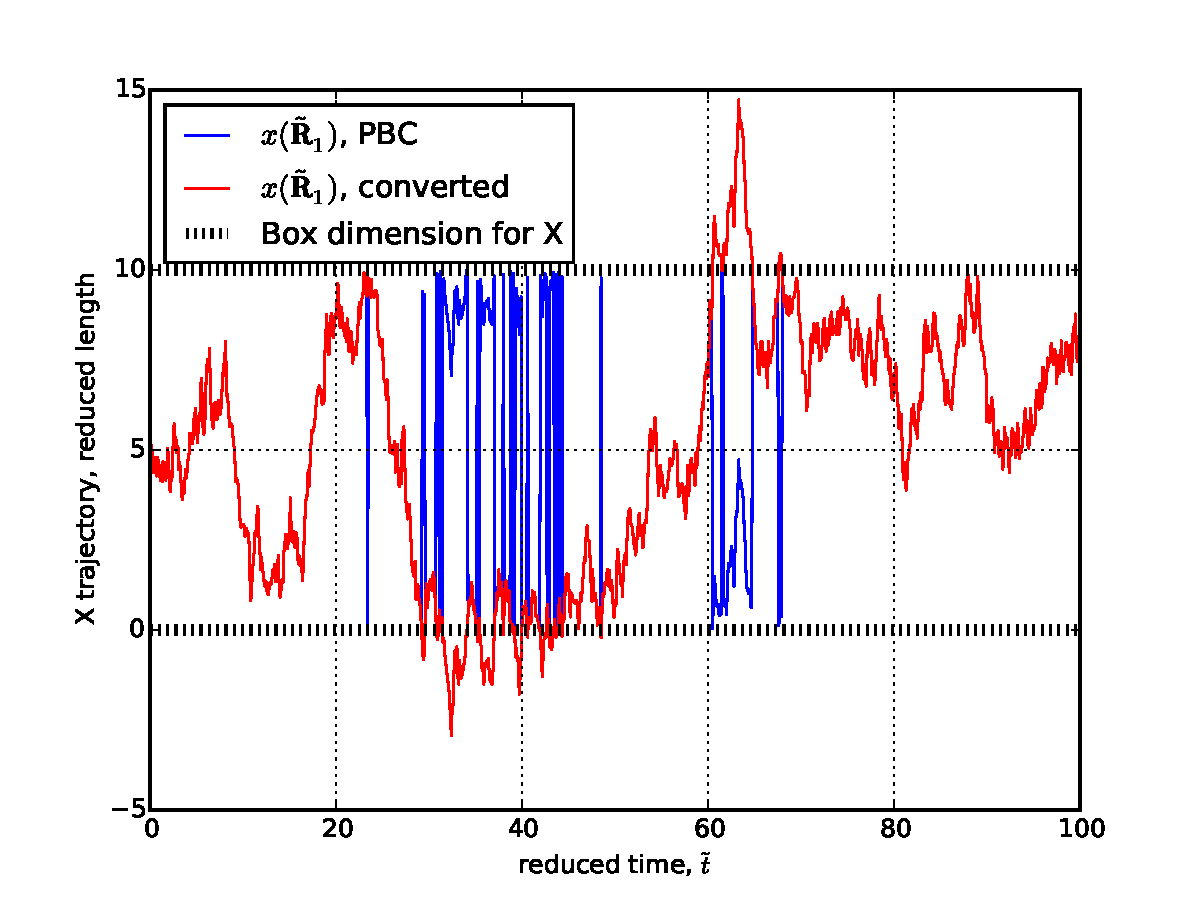
\includegraphics[width=\textwidth]{figures/converting_trajectory.pdf}
\caption{Test results for trajectory conversion. Blue color represent the trajectory using periodic boundary condition (PBC) and the red color represent the converted data. The test is done using pure Brownian motion with 100 reduced time step, and trajectory is involved only for x-coordinate of the first beads among 100 beads on the system.}
\label{fig:traj_conv}
\end{figure}

\subsection{Mean-Square Displacement for Trajectory}
First of all, it would be notice that we use simple Euler integrator that only works for pure configurational space. Therefore, we do not has any velocity information, and the velocity effect is only given by flow field of solution. On this regards, we cannot trace all the velocity profile of beads, that make difficulties to identify the equilibrium condition of Brownian motion using velocity autocorrelation function. However, the results of the Green-Kubo relation should be hold since the system only account for pure Brownian system. (NEED REINFORCEMENT) Since long-time average for the MSD has linear with respect to time, the slope gave us the diffusion coefficient, $D = k_BT/\zeta$. Recall the reduced time, equation \eqref{eq:characteristic_time}, we have
\begin{equation}
t_c = \frac{R_0^2}{D}.\label{eq:characteristic_time_D}
\end{equation}
In dimensional form, the MSD has the form of
\begin{equation}
\lim_{t\to\infty}\langle \left(\mathbf{r}_i(t)- \mathbf{r}_i(0)\right)^2\rangle_i = 2N_D Dt,
\end{equation}
where $N_D$ is spatial dimension.
Combined with equation \eqref{eq:characteristic_time_D}, the dimensionless form for MSD becomes
\begin{equation}
\lim_{\tilde{t}\to\infty}\langle \left(\tilde{\mathbf{r}}_i(\tilde{t})- \tilde{\mathbf{r}}_i(0)\right)^2\rangle_i = 2N_D\tilde{t}.
\end{equation}

\end{appendices}



\printbibliography



\end{document}
